\section{Das Schienennetz der LEAG}

Essentiell für den Betrieb der Kraftwerke ist die regelmäßige und zuverlässige Belieferung mit Braunkohle. Zu diesem Zweck betreibt die LEAG  ein Schienennetz von 391 Kilometern Länge \cite{hertzer_eisenbahner_2018}. Es verbindet die Tagebaue \emph{Jänschwalde}, \emph{Welzow-Süd}, \emph{Nochten} und \emph{Reichwalde} mit den Braunkohlekraftwerken \emph{Jänschwalde}, \emph{Boxberg} und \emph{Schwarze Pumpe}. Außerdem ist der Kohleveredelungsbetrieb in \emph{Schwarze Pumpe} angeschlossen \cite{noauthor_tagebau_2023}. Gleichzeitig fahren bis zu 25 Kohlezüge auf dem Netz. Sie dienen nicht nur allein dem Transport der Kohle. Ebenso befördern sie die Abfallprodukte der Kohleverstromung, Asche und Gips. Mit einer Maximalgeschwindigkeit von 50 km/h haben sie einen Bremsweg von 400 Metern. Zum Fuhrpark gehören 61 E-Loks und 14 Diesel-Loks \cite{hertzer_eisenbahner_2018}. \autoref{fig:leag-netz} zeigt das Schienennetz der LEAG und die Positionen der angeschlossenen Tagebaue und Kraftwerke.

\begin{figure}[!ht]
	\centering
	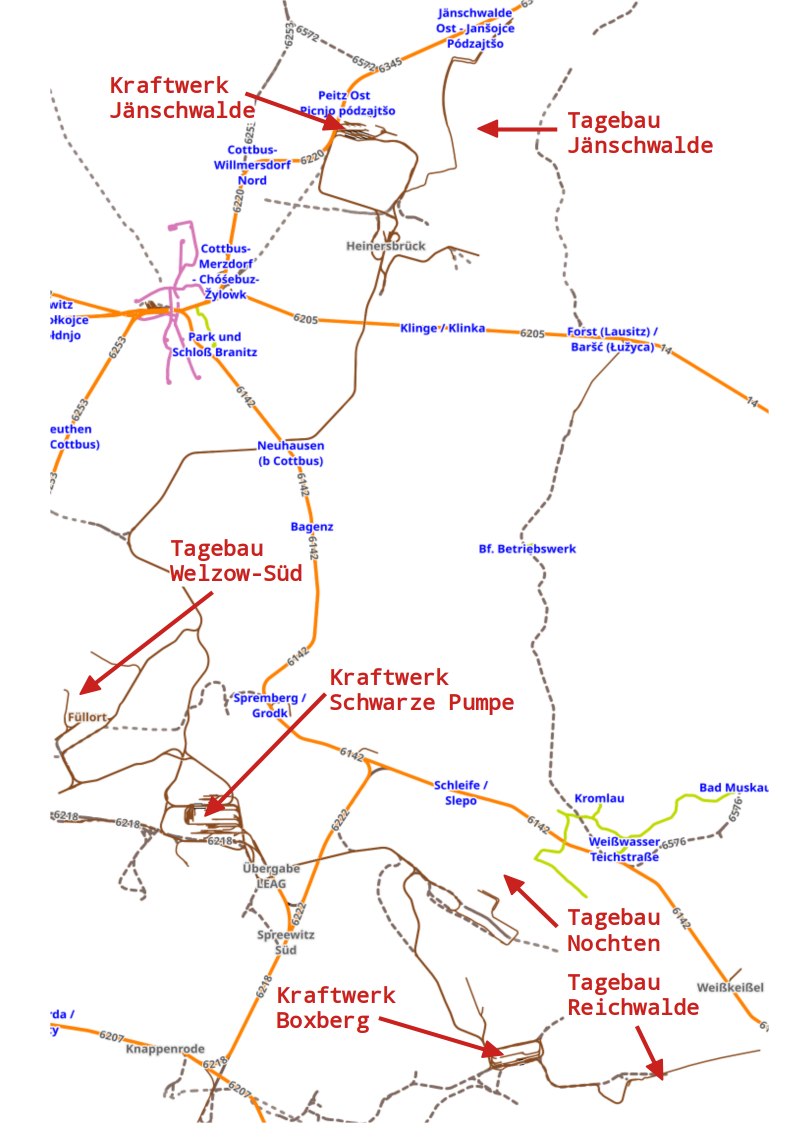
\includegraphics[width=0.75\linewidth]{images/LEAG-Netz-annotated.png}
	\caption{Das Schienennetz der LEAG für den Kohletransport (braun) und die Positionen der angeschlossenen Tagebaue und Kraftwerke (rot).}
	\label{fig:leag-netz}
\end{figure}